\documentclass[10pt,a4paper]{article}
\usepackage[latin1]{inputenc}
\usepackage{amsmath}
\usepackage{amsfonts}
\usepackage{amssymb}
\usepackage[pdftex]{graphicx}
\usepackage{float}

\begin{document}
\title{The Kuramoto-Sivashinsky Equation}
\author{Anders, Elisabeth og Espen}

\maketitle



\begin{abstract}
This is the abstract. Write smart things here.
\end{abstract}

%\begin{figure}[H]
%\centering
%\includegraphics[scale=0.5]{PDFs/IMEX/KS_plot_surface.pdf}
%\end{figure}


\section*{Introduction}
The Kuramoto-Sivashinsky equation,
\begin{equation}
\label{KSeq}
u_t + u_{xx} + u_{xxxx} + uu_{t} = 0 
\end{equation}
written in integral form as
\begin{equation*}
h_t + h_{xx} + h_{xxxx} + \frac{1}{2}h^2_x = 0, u = h_x 
\end{equation*}
is one of the simplest partial differential equations that exhibits complicated dynamics in both time and space, which is why the equation has been the attention for a lot of research. The equation was developed by two scientists at the same time in 1977 \cite{development}. Gregory Sivashinsky determined an equation for a laminar flame front, while Yoshiki Kuramoto modeled a diffusion-induced chaos using the same equation. Because of this, the equation is named Kuramoto-Sivashinsky. The KS-equation also models the motion of a fluid going down a vertical wall, e.g. solitary pulses in a falling thin film. \cite{trivia}

The reason for the complex behaviour comes from the second- and fourth-order derivatives in \eqref{KSeq}. While the second-order term acts as an energy source and has a destabilizing effect, the fourth-order term has a stabilizing effect. In addition to this, the nonlinear term transfers energy from low to high wave numbers. \cite{stabil} The KS-equation is a stiff equation, i.e. an equation where numerical methods for solving it are numerically unstable, unless the step size is extremely small. $u_{xxxx}$ is the main reason for this as it leads to rapid variation in the solution.


%Of particular interest is the case when the stiff terms are linear, which is the case of the %Kuramoto–Sivashinsky equation. Under these conditions, it may be extremely advantageous to %split the equations into its stiff and nonstiff components, and treat each of them %separately. In particular, the nonlinear, nonstiff terms are integrated using a suitable %explicit scheme, whereas the linear, stiff terms and integrated using and implicit scheme
%http://raphael.mit.edu/lcf_jp_JCP08.pdf


%http://en.wikipedia.org/wiki/Stiff_equation

%cite trivia: http://www.sciencedirect.com/science/article/pii/S0307904X11004082


%cite something: http://www.naturalspublishing.com/files/published/ed38fj6n3xt187.pdf


\section*{Numerical results}
\subsection*{Initial conditions}
In the solution of the KS-equation we had periodic boundary conditions, i.e. $u(0,t) = u(L,t)$. We also used L-periodic initial conditions. We experienced that a common initial condition used in several other reports was

\begin{equation}
\label{initialCondition}
u(x,0) = \cos(\frac{x}{16})(1 + \sin(\frac{x}{16}).
\end{equation}

We also tried the initial condition

\begin{equation}
\label{initialCondition2}
u(x,0) = \frac{1}{\sqrt{2}} \sin(x) - \frac{1}{8}\sin(2x),
\end{equation}

which worked well. The L-periodic initial conditions is customarily taken \cite{periodicInitial} to satisfy

\begin{equation}
\int_0^L\! f(x)\,\textrm{d}x = 0,
\end{equation}
which both of our initial conditions satisfy. The same article also states that for L-periodic initial data, a unique solution for \eqref{KSeq} exits, and is bounded as $t\rightarrow\infty$. The bound has been proven to be smaller than $O(L^{8/5})$. In our numerical tests, with $t=5000$, the initial condition \eqref{initialCondition} did indeed not exceed the bound, nor did \eqref{initialCondition2}.

\subsection*{Plots of the function}
The IMEX method produced figure \ref{fig:surface}.

\begin{figure}[H]
\centering
\includegraphics[scale=0.7]
{../PDFs/IMEX/KS_plot_surface.pdf}
\caption{Surface plot of the solution u(x,t)}
\label{fig:surface}
\end{figure}

As we can see, there are two parallel lines where the solution is symmetric in an interval around them. This is easier seen from the contour plot, figure \ref{fig:contour}.

\begin{figure}[H]
\centering
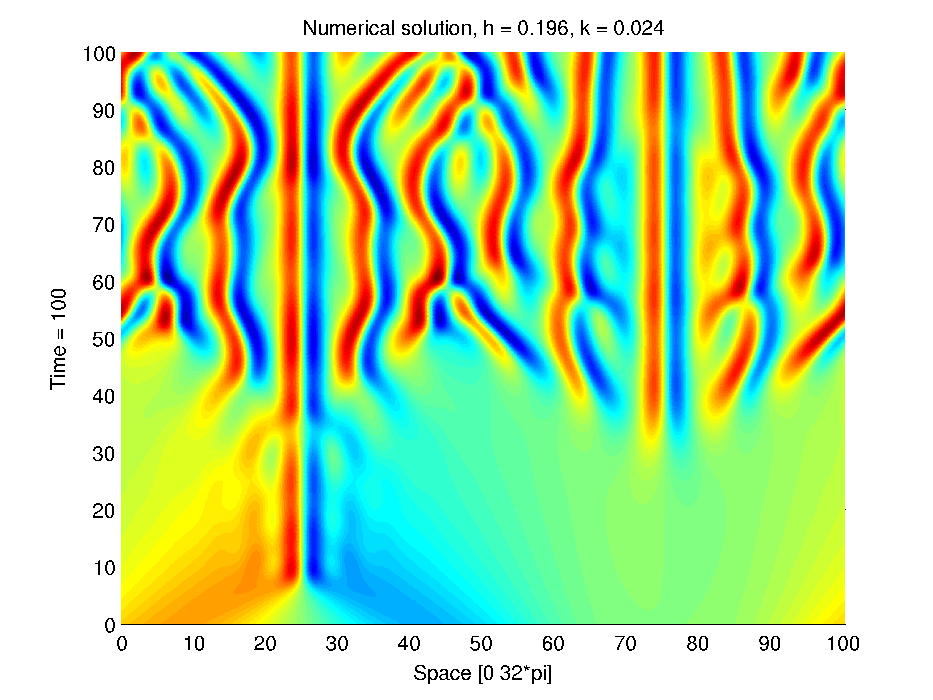
\includegraphics[scale=0.65]
{../PDFs/IMEX/KS_plot_contour.pdf}
\caption{Contour plot of the solution u(x,t)}
\label{fig:contour}
\end{figure}

Although the lines are parallel from time $t = [0,100]$, this ends after a time $t \thickapprox 250$, and it becomes even more chaotic.

Because \eqref{KSeq} has no analytical solution, we constructed a reference solution. Since our equation is stiff, we used the ODE15s solver to compute the solution, as this is particularly good for stiff systems. A semi-discretization, i.e. only discretization in space, was used in the solver. By using low values for $k$ and $h$, typically $k = 0.006$ and $h = 0.025$, we are confident that the solver produces a good approximation of the result. To see exactly how well our numerical solution is compared to the reference solution, we plotted the error between them. This produced figure \ref{fig:errPlots}.

\begin{figure}[H]
        \centering
        \begin{subfigure}[b]{0.52\textwidth}
                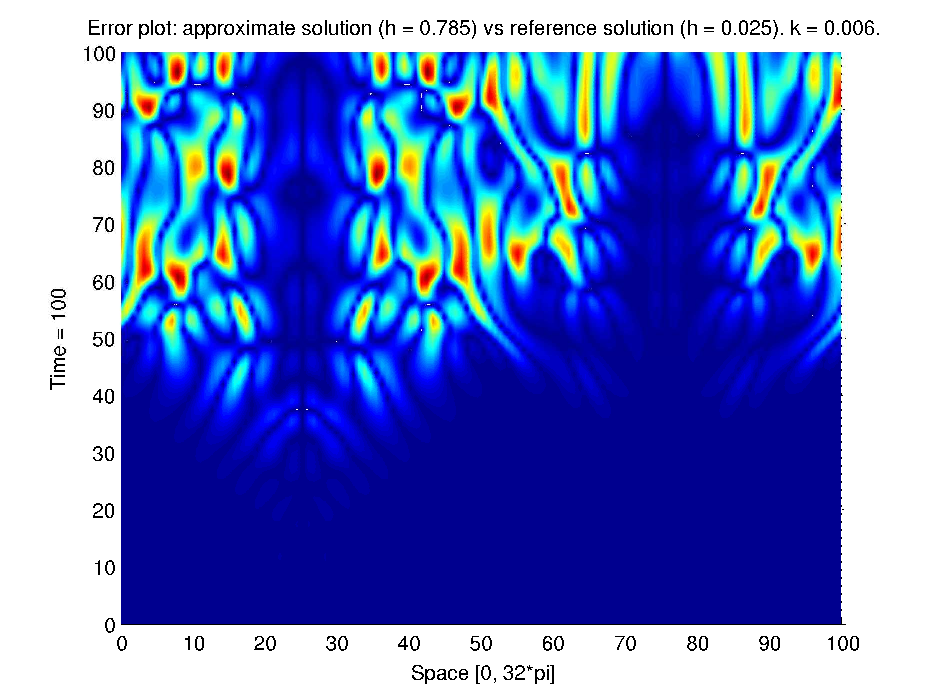
\includegraphics[width=\textwidth]{../PDFs/IMEX/error_num_ref_t100_3rd.pdf}
                \caption{Numerical solution, $h = 0.785$}
                \label{fig:highError}
        \end{subfigure}%
        ~ %add desired spacing between images, e. g. ~, \quad, \qquad etc.
          %(or a blank line to force the subfigure onto a new line)
        \begin{subfigure}[b]{0.52\textwidth}
                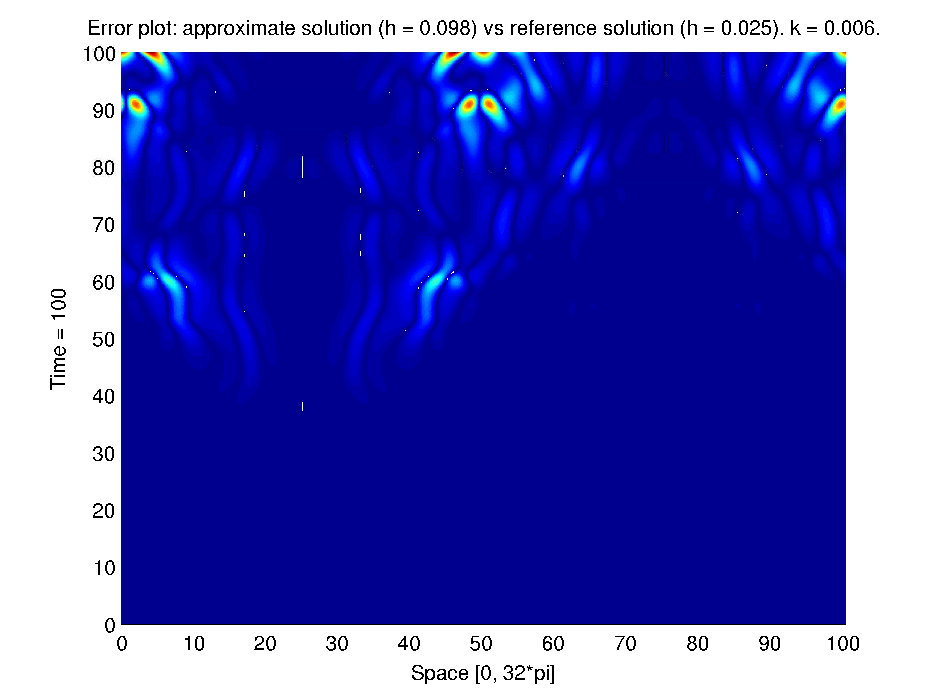
\includegraphics[width=\textwidth]{../PDFs/IMEX/error_num_ref_t100_1st.pdf}
                \caption{Numerical solution, $h = 0.098$}
                \label{fig:lowError}
        \end{subfigure}
        \caption{Comparison of the error between the reference solution and the numerical approximation for different $h$-values. Reference solution: $h = 0.025$, $k = 0.006$. Blue color shows low error, while red shows high error.}\label{fig:errPlots}
\end{figure}

As we can see, the error decreases when the $h$-value is decreased. A plot of the reference solution vs. our numerical solution, figure \ref{fig:errTime}, explains in a good way why some points have higher error than others. At the points where the reference solution and the numerical solution are out of phase, the error will naturally be large.This means a worst case error will be the sum of the amplitudes of the solutions, and this tends to happen. Worth noting is the low error at the two parallel lines, $x \thickapprox 25$ and $x \thickapprox 75$, which can also be seen in figure \ref{fig:errPlots}. 

\begin{figure}[H]
\centering
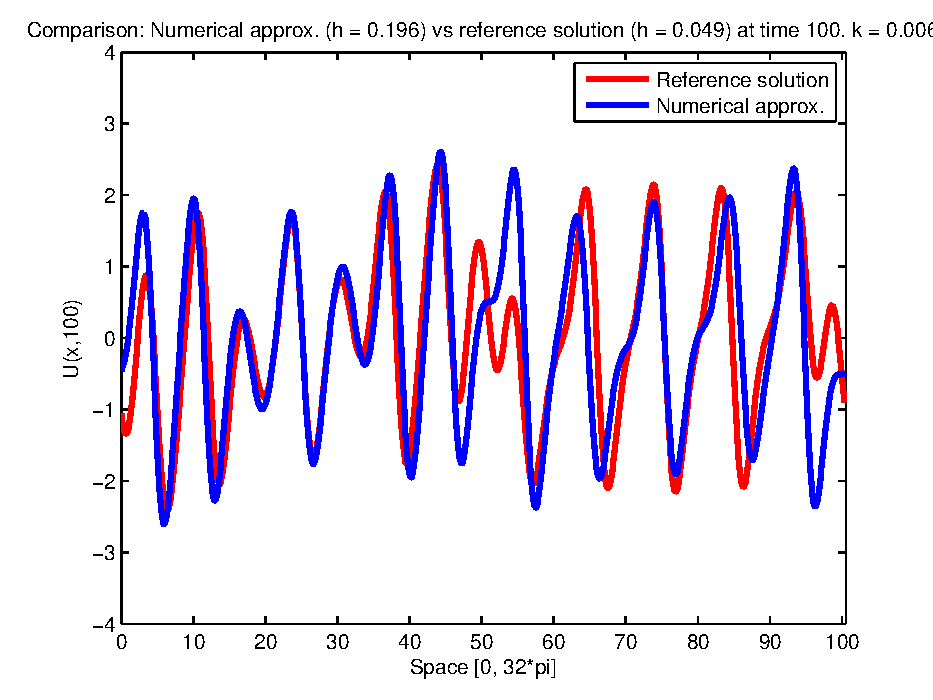
\includegraphics[scale=0.55]
{../PDFs/IMEX/comp_num_ref_t100.pdf}
\caption{Plot of $u(x,0)$ for the reference solution and the numerical solution}
\label{fig:errTime}
\end{figure}


\subsection*{Running time}

The implicit and explicit scheme both have negative and positive properties. While the explicit scheme is about 10 times faster than the implicit scheme, as shown in Figure \ref{fig:runTime}, it is has a restriction on the time step. In addition, it seems that the error is larger in the explicit scheme than the implicit scheme, independent on the number of time steps. 

\begin{figure}[H]
\centering
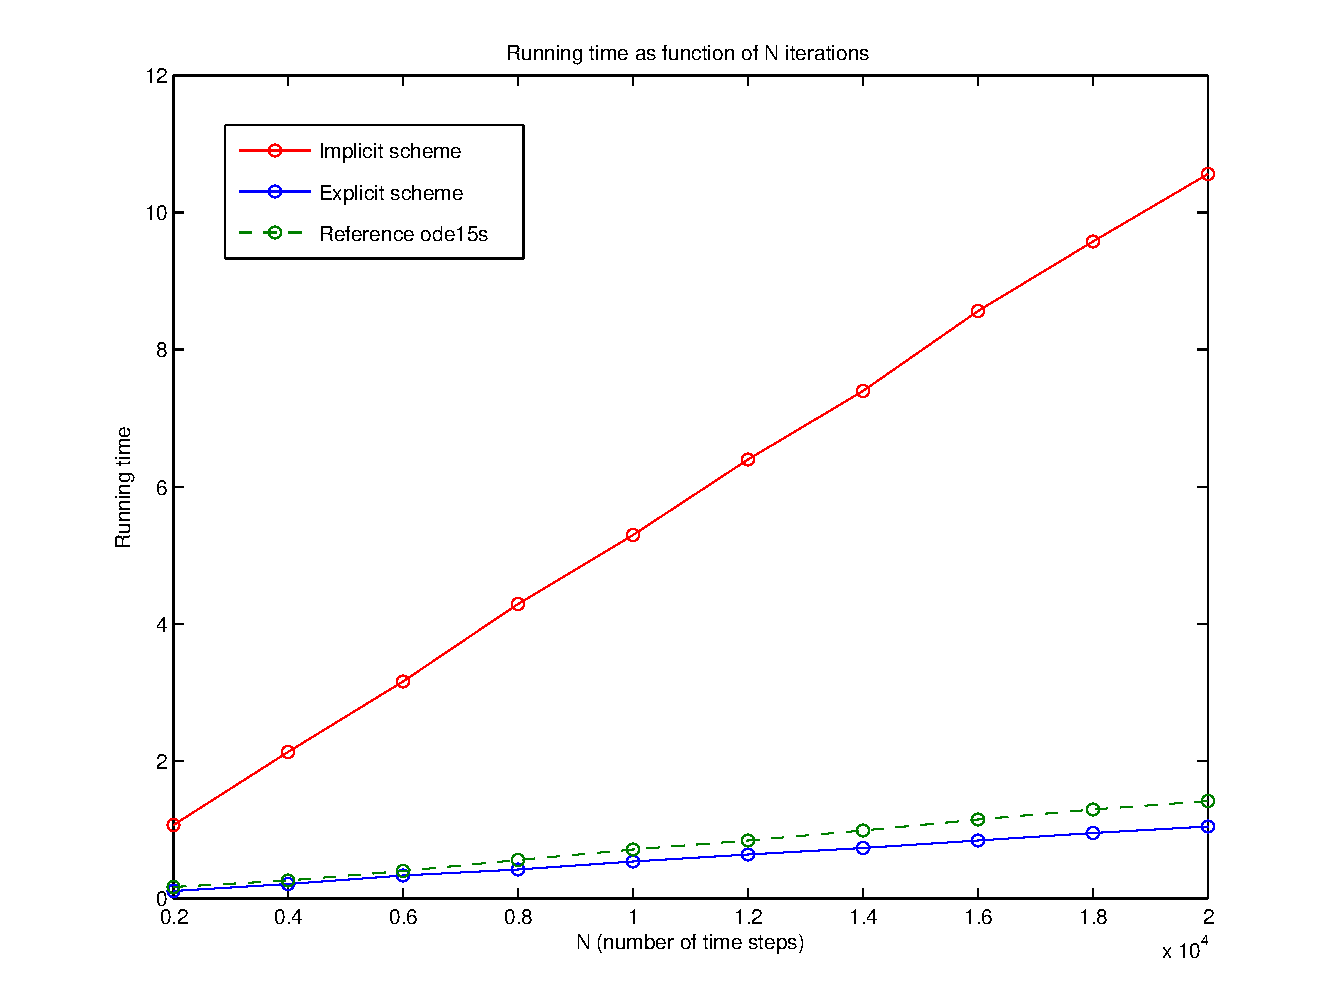
\includegraphics[scale=0.4]
{../PDFs/Comparisons/running_time3.pdf}
\caption{Running time of the two schemes as a function of time steps $N$}
\label{fig:runTime}
\end{figure}

\begin{figure}[H]
\centering
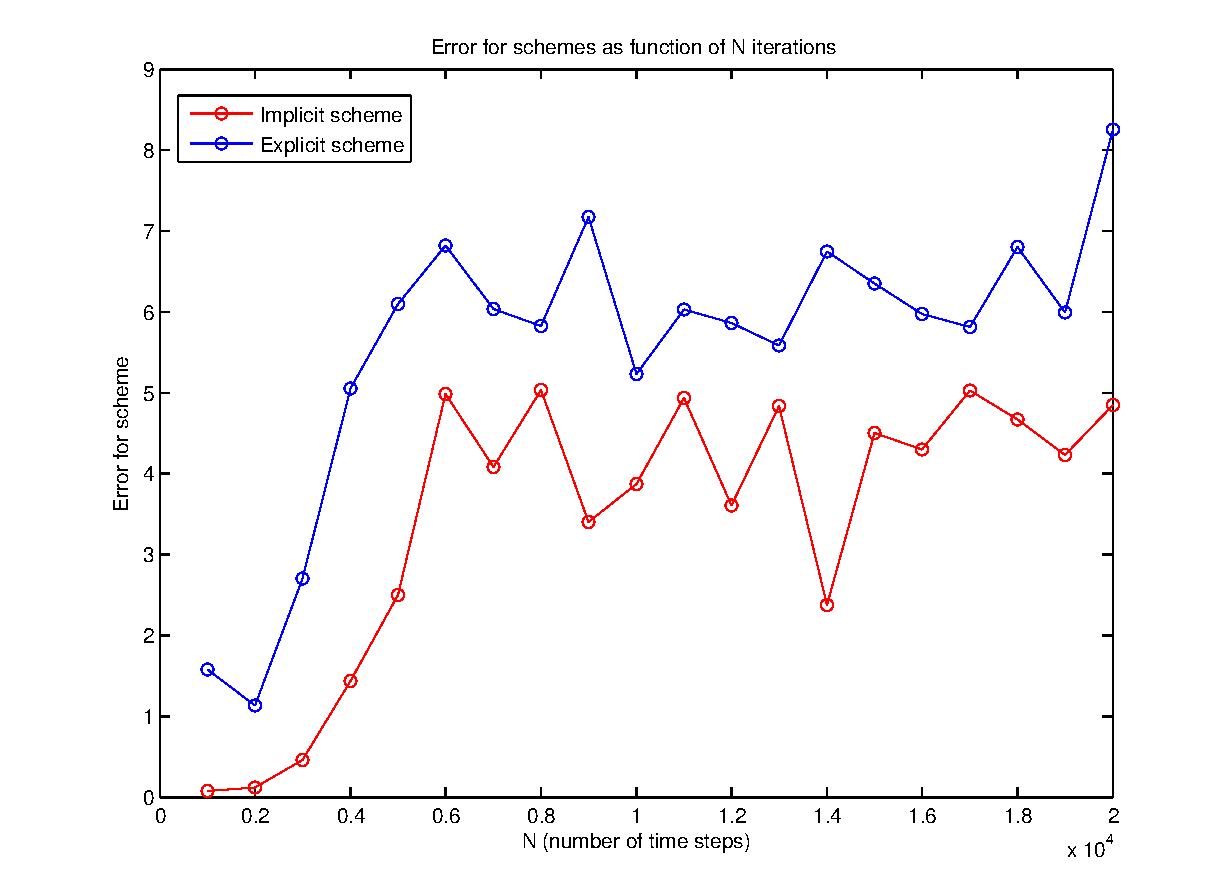
\includegraphics[scale=0.4]
{../PDFs/Comparisons/error_compare.pdf}
\caption{Running time of the two schemes as a function of time steps $N$}
\label{fig:runTime}
\end{figure}







\begin{thebibliography}{9}

\bibitem{development}
Scott Arthur Gasner, Fall 2004,
\emph{Integrating the Kuramoto-Sivashinsky equation: A simulation of the hopping state}
http://terminus.sdsu.edu/thesis\_repository/ScottGasner\_2004\_Fall\_MS\_Comp\_Sci.pdf, 03/31-2014

\bibitem{trivia}
Mehrdad Lakestani and Mehdi Dehghan, February 2012,
\emph{Numerical solutions of the generalized Kuramoto-Sivashinsky equation using B-spline functions},
http://www.sciencedirect.com/science/article/pii/S0307904X11004082, 03/31-2014

\bibitem{stabil}
Marjan Uddin and Sardar Ali, January 2013,
\emph{RBF-PS method and Fourier Pseudospectral method for solving stiff 
nonlinear partial differential equations},
http://www.naturalspublishing.com/files/published/ed38fj6n3xt187.pdf, 03/31-2014

\bibitem{periodicInitial}
Andrew Spratley, March 2010,
\emph{Kuramoto-Sivashinsky equation: A PDE with chaotic solutions},
http://www.dtic.mil/dtic/tr/fulltext/u2/a228590.pdf, 03/31-2014

\end{thebibliography}


\end{document}